\documentclass[10pt]{article}
\usepackage{natbib}
\usepackage{times}
\usepackage[T1]{fontenc}
\usepackage[utf8]{inputenc}
\usepackage[pdftex]{graphicx}
\usepackage{caption}
\captionsetup[figure]{justification=raggedright,labelfont=bf}
\usepackage{fullpage} % 1" margins
\usepackage{setspace}
\setstretch{1.5}
\usepackage{tabu}
\usepackage{xcolor}
\usepackage[backgroundcolor=yellow!30,bordercolor=yellow!30,textsize=small,textwidth=4cm]{todonotes}
\usepackage[unicode=true,colorlinks=true,urlcolor=blue,citecolor=black]{hyperref}
% \usepackage[top=2.5cm, bottom=2.5cm, outer=6cm, inner=1cm, heightrounded, marginparwidth=5cm, marginparsep=1cm]{geometry}
\usepackage[letterpaper,left=1.5cm,right=5cm]{geometry}
%\usepackage{sectsty}
%\sectionfont{\nohang\centering\normalsize\sc}   % capitalize initial letters
%\subsectionfont{\nohang\centering\normalsize\rm\em}

\renewcommand{\thetable}{S\arabic{table}}

% eat the colon so figures are labeled but have blank captions
% \makeatletter
% \renewcommand\fnum@figure[1]{\figurename~\thefigure\ignorespaces}
% \makeatother

\newcommand{\smalltodo}[2][]
{\todo[caption={#2}, size=\small, #1]
{\begin{spacing}{0.5}#2\end{spacing}}}

\newcommand{\fntodo}[2][]
{\todo[caption={#2}, size=\footnotesize, #1]
{\begin{spacing}{0.5}#2\end{spacing}}}

%% Article
\begin{document}
\raggedright
\parindent 0.5in


\begin{table}%[tbhp]
  \centering
  \small
  \caption{Global and regional sampling of clades.}
  \begin{tabu} to \textwidth {X[-3,l,b]|X[-1,r,b]X[-1,r,b]X[-1,r,b]|X[-1,r,b]X[-1,r,b]X[-1,r,b]|X[-1,r,b]X[-1,r,b]X[-1,r,b]|X[1,r,b]X[1,r,b]X[1,r,b]}
   \hline
    & \multicolumn{3}{c|}{global} & \multicolumn3{c|}{Hengduan Mountains} & \multicolumn3{c|}{Himalayas-QTP} & \multicolumn3{c}{temperate/boreal East Asia}\\
   clade                                                  & total & sampled & \% & total & sampled & \% & total & sampled & \% & total & sampled & \%  \\
   \hline
   \textit{Acer}                                          & 129   & 118     & 91 & 45    & 29      & 64 & 24    & 15      & 63 & 80    & 72      & 90  \\
   \textit{Allium}                                        & 800   & 378     & 47 & 34    & 29      & 85 & 55    & 37      & 67 & 89    & 100     & 89  \\
   Clematidinae+ Anemoninae                               & 495   & 177     & 36 & 76    & 32      & 42 & 45    & 26      & 58 & 152   & 72      & 47  \\
   Delphineae                                             & 756   & 312     & 41 & 225   & 74      & 33 & 83    & 44      & 53 & 90    & 51      & 57  \\
   \textit{Cyananthus}                                    & 66    & 47      & 71 & 41    & 28      & 68 & 26    & 24      & 92 & 14    & 10      & 71  \\
   \textit{Isodon}                                        & 100   & 63      & 63 & 55    & 40      & 73 & 20    & 9       & 45 & 36    & 24      & 67  \\
   \textit{Ligularia- Cremanthodium- Parasenecio} complex & 380   & 75      & 20 & 152   & 60      & 39 & 62    & 12      & 19 & 148   & 27      & 18  \\
   \textit{Meconopsis}                                    & 54    & 47      & 87 & 25    & 22      & 88 & 36    & 34      & 94 & 2     & 2       & 100 \\
   Microsoroideae                                         & 248   & 147     & 59 & 45    & 42      & 93 & 38    & 35      & 92 & 80    & 66      & 83  \\
   Pinaceae                                               & 234   & 226     & 97 & 34    & 32      & 94 & 26    & 24      & 92 & 63    & 63      & 100 \\
   Polygoneae                                             & 663   & 257     & 39 & 92    & 61      & 66 & 85    & 75      & 88 & 160   & 127     & 79  \\
   Primulaceae                                            & 900   & 354     & 39 & 205   & 114     & 56 & 150   & 68      & 45 & 80    & 55      & 69  \\
   \textit{Rhodiola}                                      & 70    & 57      & 81 & 32    & 28      & 88 & 37    & 30      & 81 & 34    & 20      & 59  \\
   \textit{Rhododendron}                                  & 1000  & 351     & 35 & 237   & 120     & 51 & 124   & 42      & 34 & 300   & 105     & 35  \\
   \textit{Rosa}                                          & 175   & 102     & 58 & 49    & 27      & 55 & 29    & 20      & 69 & 64    & 35      & 55  \\
   \textit{Saussurea}                                     & 416   & 147     & 35 & 108   & 73      & 68 & 130   & 63      & 48 & 157   & 56      & 36  \\
   Saxifragaceae+ Grossulariaceae                         & 760   & 313     & 41 & 209   & 54      & 26 & 155   & 45      & 29 & 170   & 102     & 60  \\
   \textit{Thalictrum}                                    & 150   & 104     & 69 & 38    & 34      & 89 & 40    & 25      & 63 & 48    & 32      & 67  \\
   \hline
    
  \end{tabu}
\end{table}

%%% Local Variables: 
%%% mode: latex
%%% TeX-master: "SI"
%%% End: 


\clearpage
\newpage

\section*{Materials and Methods}

\subsection*{Molecular dating: calibrations and topological constraints}

\noindent We followed three general guidelines in calibrating the
divergence-time analyses with node age constraints, all intended to be
conservative with respect to constraining the maximum age of any given
clade.

\begin{enumerate}

\item We used the earliest confirmed fossil record of a group to
  constrain its minimum \textit{stem} age; most fossil species are
  published based on fragmentary material that lack enough characters
  to be placed within the crown group.

\item We applied uniform priors to all calibrations.% , despite the
  % effect of inferred node age confidence intervals being larger than
  % for other commonly-used distributions, e.g.\ lognormal, exponential,
  % etc. We believe current knowledge on fossils only allow us to make
  % an assumption that one clade could originate at any time between the
  % minimum and maximum bounds.

\item We used 125 Myr, the age of the earliest eudicot fossil
  \citep{Hughes1994}, to constrain the maximum age of angiosperm
  clades in the absence of other evidence.

\end{enumerate}


\subsubsection*{Clade \fntodo{what do clade numbers refer to? can we remove them?}1. Ingroup: \textit{Allium}; outgroup scope: Amaryllidaceae}

\todo[inline]{Need a spreadsheet showing the taxa and genes (accession
  numbers) used for each BEAST analysis}

\todo[inline]{Need to add information about topological constraints in
  addition to age constraints}

\noindent There are no reliable fossils for Amaryllidaceae, so we used
secondary calibrations from a fossil-calibrated study of the
containing order Asparagales \citep{Chen2013}.

\begin{enumerate}

\item \textbf{Root age (crown of Amaryllidaceae):} 42.0--61.7 Ma. The
  bounds equal the 95\% highest posterior density (HPD) interval of
  the crown age of Amaryllidaceae from \cite{Chen2013}.

\item \textbf{Crown age of Allioideae:} 27.8--44.5 Ma. The bounds
  equal the 95\% HPD interval of the crown age of Allioideae from
  \cite{Chen2013}.\fntodo{Was Allioideae constrained monophyletic?}

\end{enumerate}

\subsubsection*{Asteraceae}

We estimated a dated backbone phylogeny of Asteraceae for the purpose
of driving secondary calibrations for clade 2, the
\textit{Ligularia-Cremanthodium-Parasenecio} complex, and clade 3,
\textit{Saussurea}, both of which lack fossils. The backbone tree
included 499 genera of Asteraceae and four outgroup genera of
Calyceraceae (SI REF)\fntodo{provide this table of taxa x genes}. Each
genus was represented by one species. We calibrated the analysis using
the following node-age constraints.

% ?? calibrations as table?
% columns: clade, node, distribution--e.g. uniform(x, y), reasoning -
% explain how the distribution was derived, with reference to fossils
% or secondary calibrations, etc.

\begin{enumerate}

\item \textbf{Crown age of Asteraceae:} \fntodo{what are the specific
    max and min ages for the constraint?}XX--YY Ma. The minimum bound
  is based on Cretaceous pollen of \textit{Tubulifloridites lilliei}
  type A, which was used to constrain of the divergence time of
  \textit{Barnadesia} and \textit{Dasyphyllum} in
  \cite{Barreda2015}. {\color{red} This is a conservative constraint,
    since the systematic position of \textit{T.~lilliei} type A within
    Asteraceae is still debated
    \citep{Barreda2015,Panero2015}}\fntodo{If the position of the
    pollen within crown Asteraceae is debatable, should the fossil
    constrain the stem, not the crown?}.

\item \textbf{Stem age of Asteraceae excluding Barnadesieae and
    \textit{Famatinanthus}:} \fntodo{125 Ma?}XX--47.5 Ma. The minimum
  bound is based on \textit{Raiguenrayum cura}, an exceptionally
  well-preserved capitulescence from the 47.5 Ma Huitrera Formation in
  Argentina \citep{Barreda2010,Barreda2012} that shares a mosaic of
  morphological characters with modern groups such as Stifftieae,
  Mutisioideae sensu lato, and Carduoideae.

\item \textbf{Stem age of Mutisieae:} \colorbox{yellow!30}{XX-YY}
  Ma. The minimum bound was set by the earliest unequivocal fossil
  pollen for Mutisieae, \textit{Mutisiapollis patersonii}, from the
  early Oligocene of Australia \citep{Macphail1994}. The pollen is
  similar to that of some extant species in \textit{Chaetanthera} and
  \textit{Mutisia}, however, it cannot be clearly placed within any
  extant genus.

\item \textbf{Stem age of Nassauvieae:} \colorbox{yellow!30}{XX-YY}
  Ma. The minimum bound was set by the earliest fossil pollen of
  Nassauvieae, \textit{Huanilipollis cabrerii}, from early Miocene
  sediments in South America \citep{Barreda2008,Barreda2010}. It is
  similar to pollen of recent \textit{Holocheilus}, \textit{Jungia},
  and \textit{Proustia}, being subprolate, tricolporate, microechinate
  and with a complex exine structure \citep{Barreda2008}.

\item \textbf{Stem age of Cichorieae excluding Scorzonerinae:}
  \colorbox{yellow!30}{XX-22} Ma. The minimum age is based on the
  earliest confirmed fossil pollen of Cichorieae, \textit{Cichorium
    intyubs}-type pollen from the Molasse of the Paratethys, which is
  at least 22 Ma old \citep{Hochuli1978}. The pollen has three poral
  lacunae, six abporal lacunae (three at each side of the equator),
  and six paraporal lacunae (three on each side of the equatorial
  ridge) \citep{Blackmore1984}, a trait combination widely distributed
  in all subtribes except Scorzonerinae \citep{Tremetsberger2013}.

\item \textbf{Stem age of \textit{Sonchus} + \textit{Launaea}:}
  \colorbox{yellow!30}{XX-YY} Ma. The minimum bound is based on
  \textit{Sonchus oleraceus}-type pollen from the Late Miocene, which
  resembles that of extant \textit{Aetheorhiza}, \textit{Hyoseris},
  \textit{Launaea}, and \textit{Sonchus} \citep{Blackmore1986}. Our
  sampling included only the latter two genera.

\end{enumerate}

\noindent We used 95\% HPD intervals for node ages in the backbone
tree as secondary calibrations for the
\textit{Ligularia-Cremanthodium-Parasenecio} complex and
\textit{Saussurea} as described below.

\subsubsection*{Clade 2. \textit{Ligularia-Cremanthodium-Parasenecio} complex}

\begin{enumerate}

\item \textbf{Root age:} 9.5--29.8 Ma.

\item \textbf{Crown age of \textit{Ligularia}:} 2.32--16.85 Ma.

\item \textbf{Crown age of \textit{Petasites} + \textit{Tussilago}}:
  1.09--15.18 Ma.

\end{enumerate}

\subsubsection*{Clade 3. \textit{Saussurea}}

\begin{enumerate}
\item Root: 2.27-13.98 Myr. % INGROUP??
\end{enumerate}

\subsubsection*{Clade 4. Ingroup: \textit{Cyananthus}; outgroup scope: Campanulaceae}

\begin{enumerate}

\item \textbf{Root age:} 62--90 Ma. The bounds are the 95\% HPD
  interval of the crown age of Campanulaceae inferred in
  \cite{Magallon2015}.

\item \textbf{Stem age of the most recent common ancestor of
    \textit{Campanula pyramidalis} and \textit{C.~carpatica}:} XX--YY
  Ma. The bounds are based on fossils of \textit{C.~palaeopyramidalis}
  \citep{Lancucka-Srodoniowa1979} which were evaluated as belonging to
  \textit{C. pyramidalis} in \cite{Cellinese2009}.
\end{enumerate}

\subsubsection{Clade 5. Ingroup: \textit{Rhodiola}; outgroup context:
  Crassulaceae}

As no reliable fossils are available for Crassulaceae, we estimated
divergence times in \textit{Rhodiola} in the context of
Saxifragales. One hundred and seventy-one species from the
Saxifragales were selected as outgroups. We applied the same fossil
calibrations as Saxigragaceae and Grossulariaceae (detailed
information see fossil calibrations for Saxifragaceae and
Grossulariaceae).

\subsubsection{Clade 6. Ingroup: \textit{Rhododendron}; outgroup context: Ericaceae}

\smalltodo[inline]{This paragraph needs to be more clear}

{\color{red}To incorporate more fossil calibrations, we selected several species
from Empetrum, Enkianthus, Erica and Kalmia as outgroups.  We mainly
use fossil calibrations for Ericaceae selected by Schwery et
al. \citep{Schwery2015}. However, to be more conservative, we
constrained the stem age rather than the crown age of Rhododendron
using the earliest fossil of this genus. This because the earliest
fossil cannot be assigned to any subgenus based on morphological
characters. We applied the earliest fossil record of Ericaceae (89.8
Myr) to be the maximum age of other calibrations in the Ericaceae.}

\begin{enumerate}

\item \textbf{Root (crown age of Ericaceae):} XX--89.8 Ma. The minimum
  bound is the the earliest fossil record of Ericaceae,
  \textit{Paleoenkianthus sayrevillensis} \citep{Nixon1993}.

\item \textbf{Stem age of \textit{Rhododendron}:} 56--89.8 Ma. The
  minimum bound is the earliest fossil record of the genus,
  \textit{R.~newburyanum} from the Paleocene of South England
  \citep{Collinson1978}. The maximum is from constraint 1.

\item \textbf{Stem age of \textit{Erica}:} 5.33--89.8 Ma. The minimum
  age of the stem of Erica was constrained by the earliest fossil
  record of this genus, E. palaeoarborea from the late Miocene of
  Europe \citep{VanderBurgh1987}. The maximum is from constraint 1.

\item \textbf{Stem age of \textit{Empetrum}:} 11.62--89.8 Ma. The
  minimum bound is the earliest fossil record of this genus, from the
  middle Miocene of Denmark \citep{Friis1979}. The maximum is from
  constraint 1.

  Stem of Kalmia: The minimum age of the stem of Kalmia was
  constrained by the earliest fossil record of this genus, K. saxonica
  from the early Miocene of Germany \citep{VanderBurgh1987}. The age
  range was set to 15.97--89.8 Myr.
\end{enumerate}
Clade 7: Isodon (Lamiaceae)

The divergence time of Isodon has been well estimated using fossil
calibrations by Yu et al. \citep{Yu2014}. We used the stem and crown
ages of Isodon to calibrate our phylogeny. The stem age of Isodon was
set to 17.03--39.84 Myr and the crown age was set to 14.66--26.44 Myr
\citep{Yu2014} using uniform priors.

Clade 8: Meconopsis (Papaveraceae)

There is no reliable fossils are available for Meconopsis and
Papaveraceae. Xiao \citep{Xiao2013} estimated the divergence time of
Meconopsis based on fossil calibrations from the other
Ranunculales. We used her estimated crown age 12--34 Myr as secondary
calibrations.

Clade 9: Pinaceae

Root (Crown of the Pinaceae): We applied the earliest fossil cone
assigned to Pinaceae, Eathiestrobus to constrain the minimum age of
the root of Pinaceae \citep{Rothwell2012}. The maximum age of the root
was set to 200 Ma as no putative fossils of Pinaceae before Jurassic
so far. We placed three fossil calibrations in Pinaceae selected by
Leslie et al. \citep{Leslie2012}. We also followed their settings of
the lower and upper bounds \citep{Leslie2012}, but use uniform priors.

Stem of Larix: The earliest reliable Larix fossil record,
L. altoborealis from middle Eocene of Canada was used to constrain the
stem age of Larix \citep{LePage1991}. The age range was
set to 41-60 Myr \citep{Leslie2012}. 

Stem of Picea: Picea burtonii, the earliest reliable fossil of Picea
from the Early Cretaceous Apple Bay locality, Vancouver Island,
British Columbia \citep{Klymiuk2012} was used to constrain the stem of
Picea.  The age range was set to 133-153 Myr \citep{Leslie2012}.

Stem of Tsuga: Tsuga swedaea from the middle Eocene Buchanan Lake
formation, Axel Heiberg island \citep{Lepage2003} was used to
constrain the stem age of Tsuga. The age range was set to 41-100 Myr
\citep{Leslie2012}.

Clade 10: Polygoneae (Polygonaceae)

Stem of Polygonaceae (root): Polygonocarpum johnsonii Manchester and
O’Leary from the Maastrichtian of southwestern North Dakota, USA was
used to constrain the minimum age of the stem of Polygonaceae
\citep{Manchester2010}. The fossil fruit possesses fusiform-reticulate
venation over the wings and deeply inset intramarginal veins which are
known only in Polygonaceae \citep{Manchester2010}. This fossil
calibration was also used to constrain the stem age of Polygonaceae in
previous study \citep{Magallon2015}. The age range was set to
65.5--125 Myr.

Stem of Polygonum: The minimum age of stem Polygonum was constrained
by the earliest fruit fossil record of Polygonum from the early
Oligocene of western Siberia \citep{Dorofeev1963}. The age range was
set to 28.1--125 Myr.

Stem of Persicaria: Several Persicaria type fossil pollen records have
been reported from Paleocene of Europe \citep{Krutzsch1970,Gruas1978}
and were accepted by Muller \citep{Muller1981}. The age range was set
to 55.8--125 Myr.

Stem of Rumex: Reliable Rumex seed and fruit fossils (R. miolusaticus)
have been reported from the middle Miocene of Germany
\citep{Mai2001}. Here, we use it to constrain the minimum age of the
stem of Rumex. The age range was set to 16--125 Myr.

Crown of Muehlenbeckia: We use the 12.7 Myr old Muehlenbeckia fossil
from New Zealand \citep{Pole1993} to calibrate the minimum age of the
crown age of Muehlenbeckia. It was assembled to the extant species
M. australis \citep{Pole1993} and this classification was evaluated by
expert of Polygonaceae \citep{Schuster2013}. The age range was set to
12.7--125 Myr.

Clade 11: Microsoroideae (Polypodiaceae)

We expanded our sampling to the Polypodiaceae to incorporate more
fossil calibrations. One hundred and seventy-nine species from
Polypodiaceae were selected as outgroups. 

Root (crown of Polypodiaceae): The earliest uncontroversial fossil for
the Polypodiaceae from Eocene of Siberia, Protodrynaria takhtajanii
\citep{Vikulin1987}, was used to constrain the minimum age
of the crown of Polypodiaceae. The maximum age of Polypodaceae was
based on a secondary calibration, the uppermost bound for the
Polygrammoids \citep{Schuettpelz2009}. The root age was set
to 33.9 -77 Myr.

Crown of Drynaria: The minimum crown age of Drynaria was constrained
using the fossil of extant species, D. propinqua which was discovered
from the late Miocene flora of SW China \citep{Wen2013}. The upper
bound was set to be 66 Myr, as the genus is unlikely to origin before
the Cenozoic. The crown age of Drynaria was set to 5.3--66 Myr.

Stem of Polypodium: The minimum stem age of Polypodium was constrained
using the earliest fossil record of this genus from the early
Oligocene of Czech Republic \citep{Kvacek2001}. The stem age of
Polypodium was set to 25.6--66 Myr.

Stem of Pleopeltis: The oldest reliable fossil of Pleopeltis from the
Miocene of Dominican Republic (15.8--20.3 Myr) \citep{Schneider2015}
was used to constrain the minimum age of the stem of Pleopeltis. The
stem age of Pleopeltis was set to 15.8--66 Myr.

Clade 12: Primuloideae (Primulaceae s.s.)

We expanded our sampling to the whole Primulaceae (s. l.). Five
fossils were used as calibrations in dating the Primulaceae
phylogeny. 

Root (Crown of Primulaceae s. l.): The minimum age of the root was
constrained by the earliest fossil record of the Primulaceae (s.l.)
assigned to Ardisia which was collected from the early Eocene London
Clay Formation (~48.6 Myr) \citep{Collinson1984}. Fossils of
Myrsinoideae have also been reported from the early Eocene United
States \citep{Irving1971}. Maximum ages of the crown age of
Primulaceae (s.l.) were constrained by the earliest fossil flowers of
the Primuloids which were collected from the Late Cretaceous
(Campanian-Maastrichtian) Mira locality of Portugal
\citep{Friis2011}. The age range of the root was set to 48.6--72 Myr.

Stem of Primuloideae (Primulaceae s.s.): The earliest fossils of the
Primuloideae which were collected from the early Oligocene Siberia was
used to constrain the minimum age for the stem of the Primuloideae
\citep{Nikitin2006}. The stem age range of Primuloideae was set to
28--72 Myr.

Stem of Primula: The earliest unequivocal fossil of Primula,
P. riosiae from the early-mid Miocene boundary was applied to
constrain the minimum age for the stem of Primula
\citep{deVos2014}. The stem age range of Primula was set to 15.96--72
Myr.

Stem of Androsace: The earliest fossil seed of Androsace was found
from the Miocene western Siberia \citep{Dorofeev1963}. We use this
fossil to constrain the minimum age of Androsace. The stem age range
of Androsace was set to 5.3--72 Myr.

Clade 13-15: Clematidinae-Anemoninae, Delphineae and Thalictroideae
(Ranunculaceae)

The fossil record of Ranunculaceae has been well reviewed by Friis et
al. \citep{Friis2011} and Pigg and DeVore \citep{Pigg2005}. The
Cretaceous record of the Ranunculaceae is sparse. For Delphinea, we
expanded our sampling to the whole Ranunculaceae. One hundred and
thirty-eight species from other genera of Ranunculaceae were selected
as outgroups.

Root (crown of Ranunculaceae): Pollen of Cretacaeisporites scabratus
from the Cretaceous (probably Late Cenomanian) of Gabon is polyporate,
showing strong affinity with pollen of some extant Ranunculaceae like
Anemone, Coptis, and Hepatica in aperture configuration and tectum
ornamentation, and also in pollen wall ultrastructure
\citep{Ward1994}. Therefore, we set the minimum age of the root based
on this fossil record. The age of the root was set to 93.9--125 Myr.

Stem of Actaea: The minimum stem age of Actaea was constrained based
on fossil fruits from the late Paleocene of North Dakota, Paleoactaea
nagelii \citep{Pigg2005}. The stem age of Actaea was set to 56.8--125
Myr.

Stem of Clematis: The minimum stem age of the stem of Clematis was
constrained based on the fossil fruits from the Oligocene Germany
\citep{Weyland1938}. The stem age of Clematis was set to 23--125 Myr.

We applied all fossil calibrations used for the Delphinae in dating
Clematidinae-Anemoninae and Thalictroideae. Besides above fossil
calibrations, we added two more calibrations. We used Eocaltha
zoophilia from the Campanian of Mexico which show similarity to seeds
of extant Caltha to constrain the stem age of Caltha
\citep{Rodriguez1998}. The stem age of Caltha was set to 70.6--125
Myr. We applied the Oligocene Ranunculus fossil fruits to constrain
the stem age of this genus \citep{Mai1985}. The stem age of Ranunculus
was set to 23--125 Myr.

Clade 16: Rosa (Rosaceae)

Rosales has very good fossil record among all the angiosperms
\citep{Xing2016}. To incorporate more fossil calibrations, we selected
203 taxa from other genera of Rosaceae and four species of Rhamnaceae
as outgroup.

Root (split between Rosaceae and Rhamnaceae): We use the old fossil
flower of Rhamnaceae from the late Campanian of Mexico, Coahuilathus
belindae \citep{Calvillo-Canadell2007} to constrain the minimum
divergence age between Rosaceae and Rhamnaceae.

Crown of subfamily Spiraeoideae (excl. Lyonothamnus, supertribe:
Kerriodae and Tribe: Neilieae): The earliest fossil from this
subfamily, Paleorosa from the middle Eocene of British Colombia
\citep{Basinger1976} was used to constrain the minimum age of this
clade as it shares feature of both the traditional subfamilies
Maloideae and Spiraeoideae. The age range was set to 49.4--125 Myr.

Crown of the Tribe Amygdleae: Prunus fossil from the middle Eocene
Okanogan Highlands \citep{DeVore2007} can be used to calibrate the
stem of Prunus. As Prunus is not monophyletic, we use this fossil to
constrain the crown of the Tribe Amygdleae. The age range was set to
49.4--125 Myr.

Crown of the Tribe Kerriae: The earliest fossil record for this tribe
is assigned to the genus Neviusia which was also discovered from the
middle Eocene Okanogan Highlands site \citep{DeVore2004}. It was used
to constrain the minimum crown age of the Tribe Kerriae. The age range
was set to 49.4--125 Myr.

Stem of Rosa: The earlies fossil record of Rosa is from the late
Eocene Florissant Formation \citep{Manchester2001}. It was used to
constrain the minimum age of the stem Rosa. The age range was set to
34--125 Myr.

\subsubsection*{Clade 17. Ingroup: \textit{Acer}; outgroup context:
  Sapindaceae}

The analysis included 118 ingroup species and 2 outgroups,
\textit{Dipteronia dyeriana} and \textit{D.~sinensis}.

\begin{enumerate}

\item \textbf{Stem age of \textit{Dipteronia}:} 60--125 Ma. The
  minimum bound is based on the earliest fossil of
  \textit{Dipteronia}, winged fruits from the Paleocene of North
  America \citep{McClain2001}. {\color{red}The maximum age was set to
    125 Ma}\fntodo{why?}.

\item \textbf{Crown age of Acer:} 47.8--125 Ma. \textit{Acer} has a
  rich fossil record, dating to at least the Paleocene
  \citep{Wolfe1987,Mai1995}. We based the minimum bound on the crown
  age on the first fossil samaras assignable to \textit{Acer} section
  \textit{Acer}, from the latest Early Eocene of North America
  \citep{Wolfe1987}. {\color{red}The maximum age was set to 125 Ma}.

\end{enumerate}

\subsubsection*{Clade 18: Ingroup: Saxifragaceae + Grossulariaceae;
  outgroup context: Saxifragales}

The analysis included 313 ingroup species and five species of
\textit{Itea} and one species of \textit{Pterostemon} as outgroups.

\begin{enumerate}
\item \textbf{Root age (crown Saxifragales):} 90--125 Ma. The minimum
  bound is based on the Turonian fossil \textit{Divisestylus}, which
  shows flowers and fruits with well-preserved morphological
  characters that indicate a clear affinity to Iteaceae
  \citep{Hermsen2003}.

\item \textbf{Stem age of \textit{Itea}:} 49--125 Ma. The minimum
  bound is based on the earliest fossil pollen assigned to \emph{Itea}
  \citep{Hermsen2013}.

\item \textbf{Stem of Ribes:} 42--125 Ma. The minimum bound is based
  on the earliest uncontroversial fossil leaves assigned to
  \textit{Ribes axelrodii} from the Eocene Bull Run floras \citep{Hermsen2005}.
\end{enumerate}

\subsection*{Biogeographical range scoring}

Data matrices for the geographic ranges of species sampled in the
studies clades were assembled mainly based on the online eFloras and
databases such as
\href{http://www.efloras.org/flora_page.aspx?flora_id=2}{Flora of
  China}, \href{http://floranorthamerica.org}{Flora of North America},
\href{http://www.efloras.org/flora_page.aspx?flora_id=5}{Flora of
  Pakistan}, \href{http://www.emplantbase.org}{EURO+MEDI PlantBase},
\href{http://plants.usda.gov}{USDA},
\href{http://www.efloras.org/flora_page.aspx?flora_id=110}{Annotated
  Checklist of the Flowering Plants of Nepal}, and
\href{http://www.gbif.org}{Global Biodiversity Information
  Facility}. We excluded records of introduced (non-native)
species. We obtained a county level distribution for most of
Himalayan-Hengduan region species by cross checking with Biodiversity
of the Hengduan Mountains database (http://hengduan.huh.harvard.edu),
dataset of distributions ranges for species included in Vascular
Plants of the Hengduan Mountains compiled by Zhang et
al. \citep{Zhang2009}, and Wu \citep{Wu2008}.

\subsection*{Ancestral regions reconstruction}

\bibliography{SI-refs}
\bibliographystyle{ecol_let}

% \begin{figure}
% \begin{center}
% 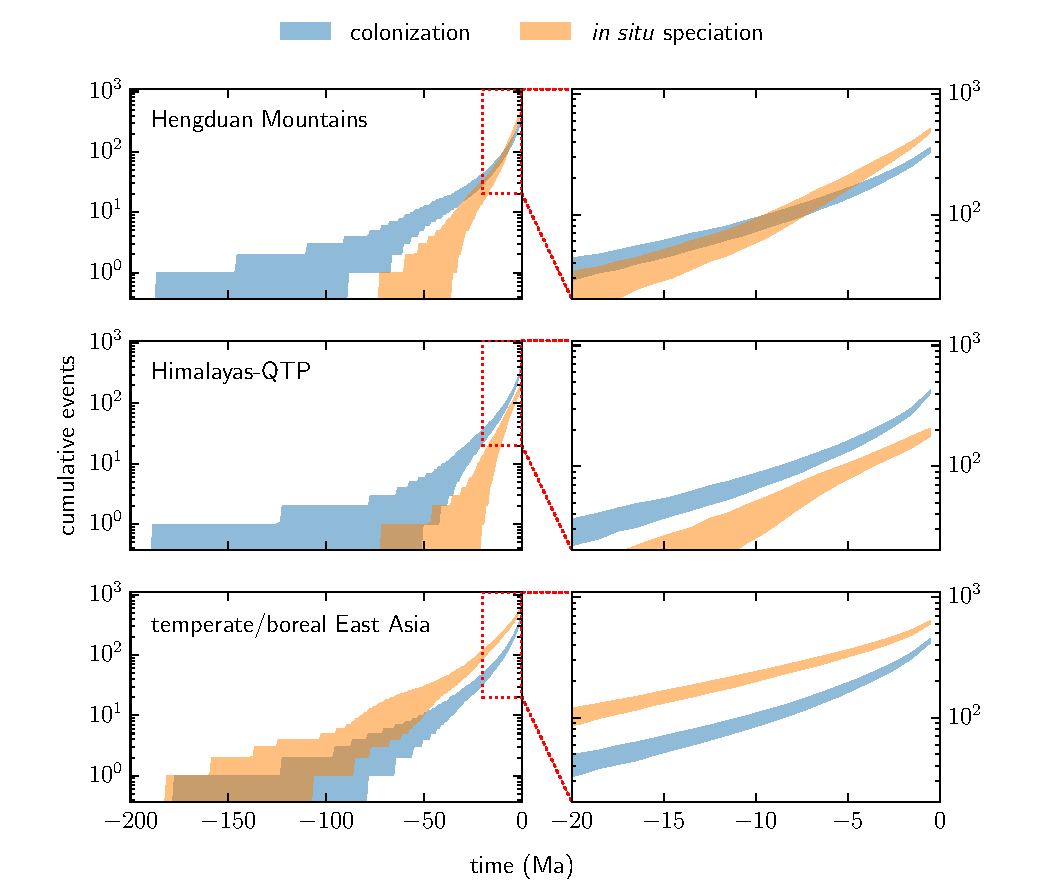
\includegraphics[width=.99\textwidth]{figures/figure_cumulative_events/figure_cumulative_events.pdf}
% \end{center}
% \caption{Assembly of regional floras by colonization and \textit{in situ} speciation events in 18 plant clades, inferred from ancestral-range reconstructions on time-calibrated molecular phylogenies. Shaded regions indicate the 5--95\% quantile intervals for the cumulative number of events through time from 500 pseudoreplicated joint biogeographic histories designed to account for phylogenetic uncertainty (see text). Panels on the right focus on the last 20 Ma, in which differences in regional assembly are most apparent. In the Hengduan Mountains region, cumulative \textit{in situ} speciation overtakes colonization about 8 Ma, whereas for the Himalayas-QTP, colonization remains the dominant process. \textit{In situ} speciation thus appears to have played a disproportionately large role in assembling the Hengduan Mountains flora since the late Miocene compared to the Himalayas-QTP, consistent with the theory of uplift-driven diversification in the Hengduan Mountains region.}
% \label{fig:cumevents}
% \end{figure}

\end{document}

%%% Local Variables:
%%% mode: latex
%%% TeX-master: t
%%% End:
